\documentclass{article}
\usepackage{graphicx}
\usepackage[margin=1in]{geometry}
\usepackage[outdir=./]{epstopdf}  					% Avoids errors when input figures
\usepackage[labelsep=period,labelfont=bf]{caption}
%\usepackage{subcaption}

\begin{document}
	\begin{figure}[tbph]
		\caption{The 10-Year Fitted Synthetic Yield of Emerging Markets} \label{fig:bsl_yQ_CI_10y_V1}
		\begin{center}								% center the minipage on the line
			\begin{minipage}{0.9\linewidth}
				\begin{center}							% center the figure inside the minipage
					\includegraphics[trim={0cm 0cm 0cm 0cm},clip,height=0.86\textheight,width=\linewidth]{../Figures/Estimation/bsl_yQ_CI_10y_V1.eps} \\
				\end{center}
				\fignotes{This figure plots the fitted synthetic yield of the emerging markets in the sample for the 10-year maturity (solid line) along with their confidence intervals equal to \(\pm 2\) standard errors (dashed lines). The standard errors are estimated using the delta method. The covariance matrix is estimated using the sample Hessian estimator calculated numerically from the joint log density.}
			\end{minipage}
		\end{center}
	\end{figure}
\end{document}
% trim = {<left> <lower> <right> <upper>}